\documentclass[a4paper]{article}
\usepackage{geometry}
\usepackage{graphicx}
\geometry{margin=0.25in}

\begin{document}
\fontsize{6pt}{0pt}\selectfont
\setlength{\abovedisplayskip}{2pt}
\setlength{\belowdisplayskip}{0pt}

\begin{minipage}{5cm}
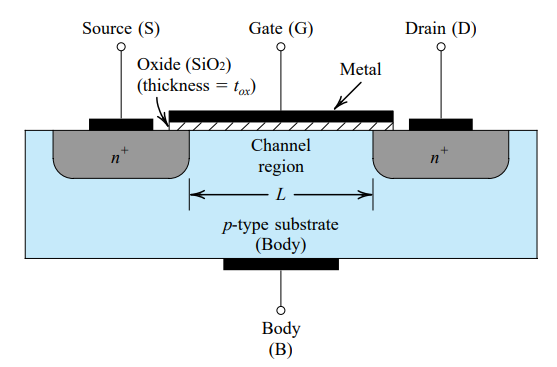
\includegraphics[width=\textwidth]{imgs/nmos}
The size of the "process" indicates the minimum
possible channel length. 

Magnitude of the electron charge in the channel [Q]:$$|Q|=C_{OX}(WL)v_{OV}$$
$C_{OX}$ is the oxide capacitance, [F/m$^2$]

$$C_{OX}=\frac{\epsilon_{OX}}{t_{OX}}$$

$\epsilon_{OX}$ is the permittivity of the SiO$_2$.\\
$t_{OX}$ is the oxide thickness.
$$i_D=\left[ (\mu_nC_{OX})\left(\frac{W}{L}\right)(v_{GS}-V_t)\right]v_{DS}$$
$$i_D=\left[ g_{DS} \right]v_{DS}$$
$$k_n^{'}=\mu_nC_{OX}$$
$$k_n=k_n^{'}(W/L)$$

When $V_{DS}$ is small, the MOSFET behaves as a linear 
resistance $r_{DS}$ whose value is controlled b the gate 
voltage $v_{GS}$.
$$r_{DS}=\frac{1}{g_{DS}}$$

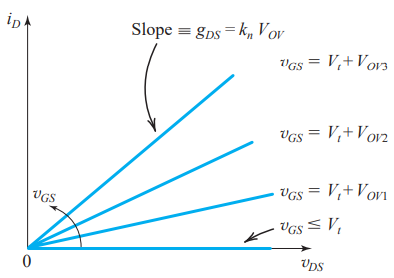
\includegraphics[width=\textwidth]{imgs/nmos_as_r}

\hrule
\vspace{1mm}
Triode vs Saturation

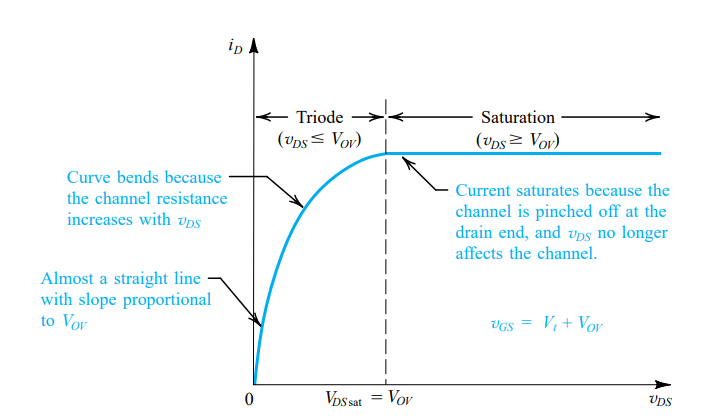
\includegraphics[width=\textwidth]{imgs/triode_sat.png}

Triode

$$i_D=k_n^{'}\left(\frac{W}{L}\right)\left(V_{OV}-\frac{1}{2}v_{DS}\right)v_{DS}$$

\end{minipage}
\begin{minipage}{5cm}
    More text over here
\end{minipage}

\end{document}